% Documento LaTeX com o artigo que estamos escrevendo

% Cabeçalho
% Onde a gente configura o documento
%%%%%%%%%%%%%%%%%%%%%%%%%%%%%%%%%%%%%%%%%%%%%%%%%%%%%%
\documentclass{article}

\usepackage[brazil]{babel}
\usepackage{graphicx}
\usepackage[round,authoryear,sort]{natbib}
\usepackage{notomath}

\newcommand{\Title}{Tectonic Insights over Victoria Land from airborne gravity and magnetic data}



% Corpo
% Onde a gente escreve o texto
%%%%%%%%%%%%%%%%%%%%%%%%%%%%%%%%%%%%%%%%%%%%%%%%%%%%%%
\begin{document}

\title{\Title}
\author{Leonardo Servan, Renata Regina Constantino Barrella}

\maketitle

\begin{abstract}
Victoria Land, located within the Transantarctic Mountains, 
features a significant rift basin that is critical for 
understanding Earth's tectonic history. This study aims to 
investigate the tectonic structure and geophysical framework of 
the region through advanced gravity and magnetic modeling using 
data from NASA’s Operation IceBridge. By analyzing airborne datasets 
alongside geological constraints, we will delineate subsurface structures, 
identify key tectonic phases, and explore the relationship between tectonic 
dynamics and geological evolution. Our findings will contribute to 
reconstructing Victoria Land's geological timeline and enhance our understanding 
of potential natural resources in the area. Additionally, this research will 
examine how tectonic variations may influence ice dynamics and their implications 
for climate change. Ultimately, this work seeks to advance knowledge of Antarctic 
tectonics and inform broader discussions on polar regions.

\end{abstract}

\section{Introduction and motivation}
\label{sec:intro}
	\subsection{Introduction and geology}
	\label{ssec:intro_geology}

	Victoria Land, a significant region along the Transantarctic Mountains, 
	hosts a major rift basin stretching from the mountain front to the western 
	margin of the Ross Sea. The basin consists of two primary sedimentary rock 
	sequences, one of Mesozoic age and the other mid- to late-Cenozoic, indicating 
	a long and complex geologic evolution. Seismic data and drill cores have revealed 
	a history of four extensional phases between 34 and 24 million years ago (Ma), 
	activating five major faults and resulting in a cumulative extension of 95 km. 
	This tectonic activity created a 145 km wide and 14 km deep basin, as described by \citet{Davey2006}.

	The geology of Victoria Land is organized into three fault-bounded tectonostratigraphic terranes: 
	the Robertson Bay, Bowers, and Wilson terranes. These terranes were accreted to the East Antarctic Craton 
	through subduction-related processes during the Paleozoic Ross Orogeny. At the Bowers-Wilson terrane boundary, 
	the Lanterman Fault marks a significant suture zone containing mafic-ultramafic rock formations and, 
	to its south, the Tonalite Belt’s calc-alkaline felsic plutons. The Wilson Terrane is also notable 
	for the Granite Harbour Intrusives, rich in hornblende-bearing, magnetite-rich quartz-granodiorites, 
	thought to be related to a Cambrian-Ordovician magmatic arc associated with subduction of the 
	paleo-Pacific plate.
	
	The Robertson Bay Terrane, a thick flysch sequence, lies adjacent to the Bowers Terrane 
	and is separated from it by the Leap Year Fault, which features the distinctive Millen Schist belt. 
	Post-accretion tectonic activity saw further subduction that contributed to significant 
	igneous intrusions, including the Devonian-Carboniferous Admiralty Intrusives, described by 
	\citet{Ferraccioli2002}. The tectonic complexity of Victoria Land, with its combination 
	of faulting, folding, and magmatic intrusions, makes it an ideal area for studies of Antarctic 
	tectonics, and has even revealed promising signs of natural resources, including gas hydrates 
	within the Victoria Land Basin and western Ross Sea \citep{Geletti2011}.

	\subsection{Motivation and justificative}
	\label{ssec:intro_motivation}

	Victoria Land offers a unique geological landscape crucial for understanding Earth’s tectonic evolution. 
	Its extensive rift basin, shaped by complex geological processes, provides vital insights into continental 
	dynamics and climate history in Antarctica. This study builds on previous research, focusing on significant 
	extensional phases that have shaped the region's sedimentary sequences.
	
	The area’s geological history, marked by substantial tectonic activity and diverse rock formations, 
	will be examined through advanced gravity and magnetic modeling. This approach will enhance our understanding 
	of subsurface structures, aiding in the reconstruction of Antarctica’s geological timeline. 
	Additionally, insights from Victoria Land’s evolution are essential for furthering the knowledge of the 
	impacts of climate change on ice dynamics and sea-level rise.
			
	Understanding the tectonic evolution of Victoria Land is crucial not only for reconstructing the geological 
	history of Antarctica but also for assessing potential resources in the area. This study aims to use 
	gravity and magnetic data collected through NASA’s Operation IceBridge to model subsurface structures 
	across Victoria Land. These airborne datasets, in combination with geological constraints and 2D forward 
	modeling, provide valuable insights into subsurface density and magnetic properties, allowing for a refined 
	understanding of the area’s tectonic framework.
	
	Ultimately, this research not only advances our knowledge of Victoria Land's 
	tectonic processes but also contributes to broader discussions about climate 
	change and its effects on polar regions. Our aim is to deepen scientific comprehension 
	of Antarctic geology and its implications for the Earth System as a whole.


\section{Objectives}
\label{sec:objectives}
The main goal of this work is to investigate the tectonic structure and geophysical framework 
of the Victoria Land region, Antarctica, through gravity and magnetic modeling, in order to 
understand the geological processes associated with rifting and their implications for the 
region's tectonic evolution. The specific objectives are:
\begin{itemize}
  \item To delineate geophysical profiles from 
  flight data over the continent and exclude the 
  oceanic region and ice shelves, ensuring the 
  modeling focuses exclusively on continental areas.
  
  \item To apply filters to remove long-wavelength 
  components of the gravity field and incorporate Moho 
  depth in the profiles, evaluating and adjusting 
  the gravity response.
  
  \item To build 2D profiles from airborne data, 
  integrating gravity and magnetic data, and refine 
  the models using geological information and 
  constraints to minimize root mean square error 
  (RMSE) and improve fit to observed values.

\end{itemize}

The scientific hypothesis is that tectonic variations in Victoria Land, 
including extensional activity and fault formation, directly influence ice dynamics, 
resulting in significant changes in melting rates and responses to global warming. 
Direct modeling with airborne gravity and magnetic data can enhance our understanding of 
these relationships.


\section{Data set}
\label{sec:dataset}
	\subsection{Gravity and magnetic anomalies}
	\label{ssec:dataset_gravmag}
	Between 2009 and 2019, the NASA Operation IceBridge Mission¹ (OIB) collected airborne remote 
	sensing measurements over Earth’s polar regions. For this study, we use data that were collected 
	during the 2013 campaign \ref{fig:flightdata}. These flights were flown at a height of ~500 m above the surface 
	at an average speed of 275 kn (142 m s–1). The gravity measurements used here were obtained with the 
	Sander Geophysics AIRGrav airborne gravity system. A 70 s temporal filter was applied to the data 
	resulting in a filter half-wavelength of ~5 km \citep{Cochran2012}. 
	
	The magnetic field is measured with a Scintrex CS-3 Cesium magnetometer and has an accuracy of 7 nT 
	\citep{Cochran2011}.

\begin{figure}[!htb] %h = here, t = top, b = bottom, ! = prioridade
	\centering
	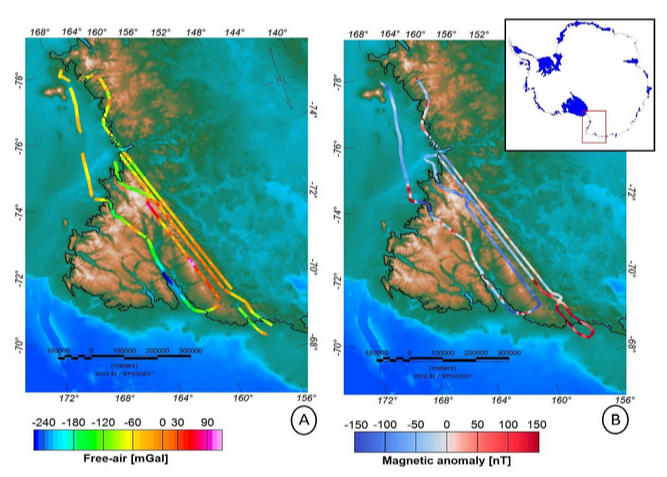
\includegraphics[width=0.5\columnwidth]{../figures/flightdata}
	\caption{
		Location map.
		a) Operation IceBridge airborne gravity data. 
		b) Operation IceBridge magnetic data.
	}
\label{fig:flightdata}
\end{figure} 

	\subsection{Constraints}
	\label{ssec:dataset_constraints}
	For the 2D models, we will use the ice thickness and bed topography that were 
	measured by the Multi-channel Coherent Radar Depth Sounder (MCoRDS) with 
	approximately 10 m accuracy (Leuschen, 2012).
	
	The method will be performed following the steps described below:
\begin{enumerate}
	\item Define the profiles based on flights so that they are positioned 
	over the continent. Modeling will not be performed over the oceanic 
	region and/or ice shelves
	\item Analyze filters to remove the long wavelength of the gravity field 
	(e.g. polynomial, low-pass, linear-regression). 
	We will also analyze the long wavelength response by adding the Moho depth 
	(e. g. \citet{An2015};\citet{Baranov2021}) into each profile.
	\item Build the 2D profiles from the airborne date. 
	The initial model will include gravity and magnetic data. 
	The geological model will have Ice surface and bedrock topography 
	from airborne radar data. Choose the densities and susceptibilities 
	for each package. Initially, average densities and susceptibilities 
	(e.g. \citet{Scheinert2016}; \citet{Augie2022} will be assigned 
	for the ice and the crust. 
	\item Refine the models using geological information over the area 
	(and possible new constraints that might appear throughout the course of the project) 
	in order to better adjust the calculated gravity and magnetic 
	with the observed values, minimizing the root mean square error (RMSE) between them.
	\item Estimating an uncertainty for the method base on previous similar works 
	(e.g. \citet{Tinto2015}; \citet{Constantino2020}).
\end{enumerate}

\section{Method}
We will perform a 2D forward model using the Geosoft GM-SYS 2D software package 
along X profiles in Victoria Land, Antarctica. 
The gravity response is calculated based on the method of \citet{Talwani1959}. 
The magnetic response is calculated based on the method of \citet{Heirtzler1964}.


% Usar o doi2bib.org para referencias
\bibliographystyle{apalike}
\bibliography{references.bib}


\end{document}